\documentclass[letterpaper, 14pt]{article}
\makeatletter
\def\sectionsuffix{.}

\renewcommand\@seccntformat[1]{\csname the#1\endcsname%
	\csname#1suffix\endcsname\quad}
\makeatother

%opening
\title{Bump detection algorithm project}
\author{Igor Trubnikov, MS}
%\date{}

\usepackage[utf8]{inputenc}
%\usepackage[english]{babel}
\usepackage{braket}
\usepackage[margin=0.5in]{geometry}
\usepackage{amsmath, amsfonts, amssymb, amsthm}
\usepackage{bbold}
\usepackage{graphicx}
\usepackage{fullpage}
\usepackage{scrextend}
\usepackage{hyperref}

\newcommand{\bd}{\textbf}
\usepackage[framed,numbered,autolinebreaks,useliterate]{mcode}

\hypersetup{
	colorlinks=true,
	linkcolor=blue,
	filecolor=magenta,
	urlcolor=cyan,
	pdftitle={Bump detection project},
}

\begin{document}

\maketitle
\tableofcontents
\newpage

\section{Introduction}
The goal of this project is to develop a high performing low-error-rate algorithm which is able to detect bump-like features on the picture. Very often bumps are associated with defects on the product of technological operation.\\
Bump-like defects can happen on electronic panels, mirrors and other surfaces.\\
Detecting of these features may also potentially be useful in analyzing geo-mapping data (on Earth as well as on Mars or Moon).\\

\newpage

\section{Description of the algorithm}

\begin{enumerate}
	\item Apply \mcode{maximum\_filter} algorithm available in Python \mcode{scipy.ndimage} package.
	\item Then find local maxima using code from \mcode{find\_local\_maxima\_np} function.
	\item Process 8 neighboring pixels for each pixel in the image.
	\item Iterate through each of a local maxima and prune the sub-maximal peaks.\\
	This extends the neighborhood, combines and prunes away unwanted maxima using the noise tolerance to decide what counts and what not.
\end{enumerate}

Following code assumes that name of input file is \bd{01\_Gray8bit.jpg} and that this image is 8-bit. It was converted to 8-bit image from the original Image1.jpg file.
\lstinputlisting[language=Python]{../bump_detect.py}
\newpage

\section{Verification}
Below are few images each representing original image as it appears after running of particular stage of algorithm.
\begin{figure}[!htbp]
	\centering
	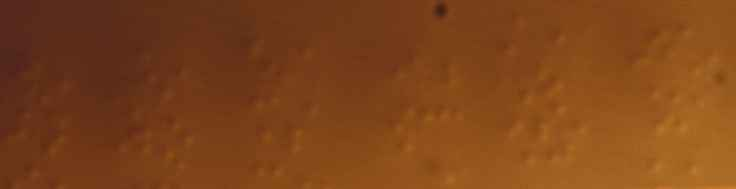
\includegraphics[totalheight=3cm]{./images/Image1.jpg}
	\caption{Original image.}
	\label{fig:origImage}
\end{figure}
\begin{figure}[!htbp]
	\centering
	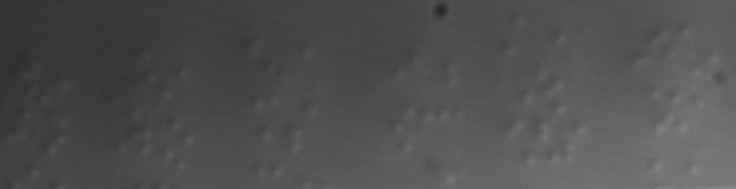
\includegraphics[totalheight=3cm]{./images/01_Gray8bit.jpg}
	\caption{Original image in gray scale 8-bit.}
	\label{fig:origImageGray}
\end{figure}
\begin{figure}[!htbp]
	\centering
	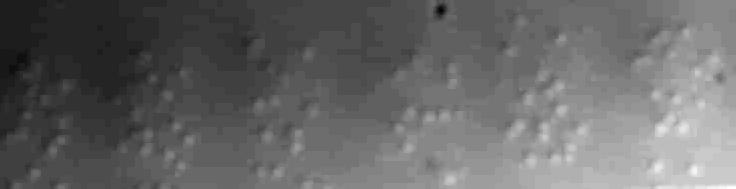
\includegraphics[totalheight=3cm]{./images/02_maxFlt.jpg}
	\caption{Image after applying \mcode{maximum\_filter}.}
	\label{fig:maxFltImage}
\end{figure}
\begin{figure}[!htbp]
	\centering
	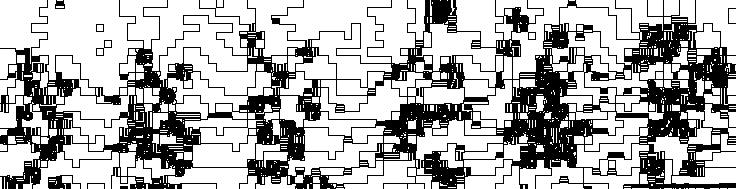
\includegraphics[totalheight=3cm]{./images/03_LocalMax.jpg}
	\caption{Binary image after applying local maxima technique.}
	\label{fig:localMaxImage}
\end{figure}
\begin{figure}[!htbp]
	\centering
	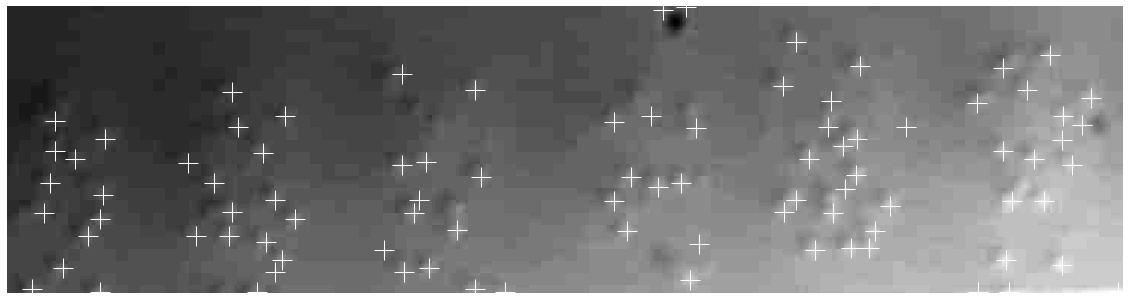
\includegraphics[totalheight=3cm]{./images/04_FinalBumps.jpg}
	\caption{Final image after run of algorithm with cross marks on the detected bumps.}
	\label{fig:finalImage}
\end{figure}
\newpage

\section{Conclusion}
Algorithm presented above is not universal. It produces false positives in some cases.\\
The best feature of the algorithm is a usage of \mcode{maximum\_filter}.\\\\
Other techniques worse trying are:
\begin{itemize}
	\item Try to split original image in few parts and analyze those parts separately.\\
	Then combine bumps from different parts.\\
	Splitting image will help to reduce the effect that one part of the image is much brighter then another.\\
	And uneven brightness negatively affects algorithm.
	\item Use histogram equalization before running algorithm. I tried and it did not go well.\\
	Adaptive histogram equalization did not help either.
\end{itemize}

\end{document}
